\documentclass[11pt, a4paper, fleqn]{article}

\usepackage[portuguese]{babel}
\usepackage{graphicx}
\usepackage{leading}
\usepackage{tabularx}
\usepackage{geometry}
\usepackage[utf8]{inputenc}
\usepackage{booktabs}
\usepackage{array}

%----------------- font -------------------------------------------------------%
\usepackage[T1]{fontenc}
\usepackage{paratype}
\usepackage[basic, italic]{mathastext}

%----------------- titles formats ---------------------------------------------%
\usepackage{titlesec}
\titleformat{\part}
{\LARGE\bfseries}{\thepart}{1em}{}
\titleformat{\section}
{\LARGE\bfseries}{\thesection}{1em}{}
\titleformat{\subsection}
{\Large\bfseries}{\thesubsection}{1em}{}
\titleformat{\paragraph}[runin]
{\sffamily\bfseries}
{}
{0pt}
{}

%----------------- footnote format --------------------------------------------%
\usepackage[perpage, bottom, marginal]{footmisc}
\makeatletter
\renewcommand{\@makefnmark}{\hbox{\textsuperscript{\sffamily\@thefnmark}}}
\makeatother
\renewcommand*{\footnotelayout}{\footnotesize\sffamily}

%----------------- page number format -----------------------------------------%
\usepackage{fancyhdr}
\fancypagestyle{pagestyle}{%
	\fancyhf{} % clear all header and footer fields
	\fancyfoot[C]{\makebox[\textwidth]{\sffamily\normalsize\thepage}} % centered footer
	\renewcommand{\headrulewidth}{0pt}
	\renewcommand{\footrulewidth}{0pt}
}

%----------------- verbatim ---------------------------------------------------%
\usepackage{fancyvrb}

\begin{document}
	\sffamily
	\setlength{\parindent}{0em}
	\emergencystretch 3em
	\renewcommand{\baselinestretch}{1.25} 
	
	\begin{titlepage}
		
\includegraphics[width=26mm]{imgs/UM.jpg}
\includegraphics[width=26mm]{imgs/EE.jpg}
		
		\vspace{7mm}
		\leading{17pt}
		{\Large
			\textbf{Universidade do Minho}
			\\
			{\fontseries{l}\selectfont
				Escola de Engenharia
		}}
		
		\vspace{50mm}
		\leading{27pt}
		{\huge
			\textbf{Sistemas Distribuídos}
			\\
			Trabalho Prático
		}
		\\
		%
		\\
		{\LARGE
			Licenciatura em Engenharia Informática
			\\
			Ano Letivo 2025/2026}
		
		\vspace{22mm}
		\leading{15pt}
		{\Large
			\begin{tabularx}{\textwidth}{@{}p{20mm} X}
				\multicolumn{2}{@{}l}{\textbf{Grupo 18}} \\
				\multicolumn{2}{@{}l}{} \\
				100751 & Diogo Luís Barros Costa \\
				106919 & Eduardo Freitas Fernandes \\ 
				106842 & Gonçalo Rodrigues Ribeiro \\
				106888 & José Mário Raimundo Lima \\
			\end{tabularx}
		}
		
		\vspace*{\fill}
	\end{titlepage}
	
	\newgeometry{left=25mm,right=20mm,top=25mm,bottom=25mm}
	\setlength{\parindent}{1em}
	
	\tableofcontents
	
	
	
	\section{Apresentação}
	
	Neste trabalho prático, desenvolvido no âmbito da unidade curricular de \textbf{Sistemas Distribuídos}, tem como principal objetivo a implementação de um \textbf{serviço distribuído para o registo e consulta de eventos organizados em séries temporais}. O sistema permite armazenar informação relativa à \textbf{venda de produtos} e disponibilizar operações de \textbf{agregação}, \textbf{filtragem} e \textbf{notificação de ocorrências} sobre dados históricos.
	
	A solução adotada segue uma arquitetura \textbf{cliente-servidor}, na qual um \textbf{servidor central} é responsável por gerir a informação e responder a pedidos submetidos por múltiplos clientes através de \textbf{sockets TCP}. O sistema foi concebido para funcionar num \textbf{ambiente concorrente}, suportando pedidos de vários clientes em simultâneo e permitindo que cada cliente possa efetuar \textbf{múltiplos pedidos concorrentes}, sem bloqueios indesejados.
	
	Atendendo ao \textbf{potencial elevado volume de dados}, foram implementados mecanismos de \textbf{persistência em disco} para armazenar séries temporais de dias anteriores. As operações de agregação são avaliadas de forma \textit{lazy}, sendo os resultados \textbf{calculados apenas quando solicitados} e armazenados numa \textbf{cache com política LRU}, de modo a limitar o uso de memória e a \textbf{melhorar o desempenho global do sistema}.
	
	
	\section{Arquitetura Geral}
	
	O código fonte apresentado na diretoria \texttt{SalesTrace} está dividido em três secções: \textbf{Servidor}, \textbf{Cliente} e \textbf{Scripts auxiliares}. Nos ficheiros auxiliares dispomos de uma classe em Java (\texttt{Tests.java}) que executa testes de performance sobre o servidor (estes testes são discutidos na secção \textbf{Avaliação Experimental}).
	
	Nos módulos de execução do \textbf{Cliente}, dispomos de uma interface simples mas funcional sobre a linha de comandos (\texttt{SalesTraceClientMain.java}). Esta interface dá uso à Interface \texttt{ISalesTraceClient} que por sua vez é implementada pela classe \texttt{SalesTraceClient}. Esta biblioteca é multithreaded e disponibiliza as operações do servidor a um cliente.
	
	A secção do \textbf{Servidor} é a mais complexa, pois é suportada pelos seguintes módulos:
	\begin{itemize}
		\item \texttt{SalesTraceServer}: classe que valida informação e resolve pedidos vindos de clientes
		\item \texttt{ClientHandler}: trata da conexão com um cliente e aplica o protocolo de comunicação estabelecido
		\item \texttt{LastDaysManager}: gestor que disponibiliza operações sobre os dias anteriores
		\item \texttt{ClientsManager}: gestor da informação dos clientes, que regista e valida estes
		\item \texttt{LRUCache}: cache LRU de agregações de informação thread safe.
	\end{itemize}
	
	Existem também certas classes imutáveis que assitem estes módulos, como: \texttt{Event}, \texttt{CacheKey}, \texttt{ClientInfo}, \texttt{QueryType} e \texttt{RequestType}.
	
	
	\section{Funcionalidades do Serviço}
	
	\subsection{Registo de Eventos}
	
	Uma vez que vários clientes podem adicionar eventos simultâneamente, esta funcionalidade envolve o acesso concorrente a um estado partilhado no servidor. Para garantir consistência dos dados e evitar condições de corrida, a inserção de eventos é realizada dentro de secções críticas protegidas por mecanismos de exclusão mútua, isto é, a série temporal do dia atual (\texttt{List<Event>}) é protegida por um \texttt{ReentrantLock}.
	
	
	\subsection{Agregação de Informação}
	
	Todas as agregações disponibilizadas pelo sistema partilham o mesmo comportamento funcional. Uma thread necessita de analisar uma sequência de dias, logo efetua um pedido ao módulo \texttt{LastDaysManager} pela série temporal do dia x. Após o tratamento dessa série, a thead indica ao gestor que já não necessita da série através do método \texttt{releaseEvents(int d)}. Este mecanismo permite que várias threads consumam a mesma série temporal, mas ao mesmo tempo garante que não existem mais de \texttt{S} séries em memória. As séries temporais do dias passados são imutáveis, logo várias threads podem ler estes recursos de forma concorrente, contribuindo para um grau elevado de paralelistmo, aumentando a escalabilidade do sistema. Se já existirem S séries em memória, a thread que necessita do recurso terá que entrar numa espera (através de \texttt{Condition.awai()} até que exista um lugar livre para a série desejada.
	
	Os resultados das agregações são guardados numa cache LRU, acessível através do nome do produto, número de dias e tipo de agregação. Esta cache é protegida por mecanismos de exclusão mútua, de forma a manter a consistência do sistema.
	
	
	\subsection{Filtragem de Eventos}
	
	A funcionalidade de filtragem de eventos distingue-se das restantes funcionalidades do sistema por devolver listas potencialmente extensas de eventos, o que introduz desafios ao nível do volume de dados trasmitidos entre cliente e servidor. Esta operação utiliza os mesmos mecanismos que as agregações. A thread atribuida efetua um pedido ao recurso desejado (a série do dia desejado) e filtra os eventos dos produtos. Após o tratamento necessário, indica ao gestor que já não necessita da série. A serialização eficiente está descrita na secção do \textbf{Protocolo de Comunicação}.
	
	
	\subsection{Notificação de Ocorrências}
	
	A funcionalidade de notificação de ocorrências permite que os clientes sejam informados quando determinados padrões de vendas são verificados, como vendas simultâneas ou consecutivas. Estas operações assumem um comportamento bloqueante, permanecendo ativas até que a condição seja verificada. Esta sincronização é realizada através de mecanismos de espera condicional (\texttt{Condition}), permitindo que uma thread suspenda a sua execução até ser explicitamente acordada.
	
	Após um cliente adicionar um evento ao dia corrente, as threads que esperam por notificações são sinalizadas e verificam se a sua condição foi satisfeita. Para a notificação de vendas consecutivas, a thread percorre a série verificando se exitem vendas consecutivas de produtos. Para a notificação de vendas simultâneas, a thread percorre a série à procura dos produtos selecionados.
	
	
	\subsection{Mudança de Dia}
	
	A mudança de dia é distribuida por três secções do servidor: no módulo dos dia corrente, da cache de agregações e dos dias passados. Esta operação deve ser atómica, não permitindo que outras operações sejam feitas concorrentemente. Através desta análise do facto de esta operação ser pouco frequente, dá-mos uso a um \texttt{ReadWriteLock} para esta operação.
	
	Esta operação começa por colocar a série do atual em disco, através de uma serialização binária simples:
	\begin{itemize}
		\item nome do produto (\texttt{writeUTF()})
		\item quantidade (\texttt{writeInt()})
		\item preço de venda (\texttt{writeFloat()})
	\end{itemize}
	O segundo passo é esvaziar a cache de agregações, e por fim indicar ao gestor dos dias anteriores a existência de um novo dia.
	
	
	\section{Protocolo de Comunicação}
	
	Cada mensagem trocada entre servidor e cliente está marcada com um tipo, que permite a ambos identificar o contexto da mensagem. Em cada mensagem é reservado um \textbf{byte} para o seu tipo. Na tabela \ref{tab:tipos} estão apresentados os tipos de mensagens.
	\begin{table}[htbp]
		\centering
		\caption{Tipos de mensagens}
		\label{tab:tipos}
		
		\newcolumntype{Y}{>{\centering\arraybackslash}X}
		
		\begin{tabularx}{\textwidth}{Y Y}
			\toprule
			\textbf{Tipo} & \textbf{Sigla} \\
			\midrule
			Autenticação & LOG IN \\
			Registo & SIGN IN \\
			Adicionar Evento & ADD EVENT \\
			Quantidade de Vendas & STOCK \\
			Volume de Vendas & TOTAL \\
			Preço Médio & AVERAGE \\
			Preço Máximo & MAXIMUM \\
			Filtrar Eventos & FILTER \\
			Vendas Simultâneas & SIMULTANEOUS \\
			Vendas Consecutivas & CONSECUTIVE \\
			Mudar de Dia & NEXT DAY \\
			Erro & ERROR \\
			\bottomrule
		\end{tabularx}
		
	\end{table}
	
	
	\subsection{Cliente}
	
	Na mensagem de \textbf{Autenticação} o cliente envia o nome de utilizador e password. Ambos estes elementos são strings, logo terão comprimentos variáveis, então é necessário indicar o comprimento da string, seguido do seu conteúdo. A função \texttt{writeUTF()} é usada para este tipo de serialização.
	
	A mensagem é semelhante para o \textbf{Registo} de um cliente. O nome de utilizador e palavra passe são enviados, mas também um \textbf{boleano} que indica se o cliente é administrador ou não.
	
	Para \textbf{Adicionar um Evento} o cliente indica o nome do produto, numa string, a quantidade, num inteiro, e o preço da venda, num float.
	
	No cálculo de \textbf{Agregações de Informação}, a mensagem enviada é igual nos 4 tipos (\texttt{STOCK TOTAL AVERAGE MAXIMUM}). O cliente deve enviar o nome do produto, representado numa string, e o número de dias anteriores, num inteiro.
	
	Na \textbf{Filtragem de Eventos} o utilizador indica o dia que deseja filtrar (através de um inteiro), o número de produtos que o conjunto de produtos tem (através de um inteiro), e o conjunto do nome dos produtos (através de uma sequência de strings).
	
	Para a notificação de \textbf{Vendas Simultâneas} o cliente indica o nome do primeiro produto (numa string) e o nome do segundo produto (também numa string). A mensagem de notificação de \textbf{Vendas Consecutivas} é composta apenas pelo número de vendas consecutivas, através de um inteiro.
	
	No pedido de \textbf{Mudança de Dia} o cliente não necessita de indicar nenhuma informação extra.
	
	
	\subsection{Servidor}
	
	Na resposta às mensagens de \textbf{Registo} e \textbf{Autenticação}, enviadas pelo cliente, o servidor envia um boleano, que indica se o registo/autenticação teve sucesso, e um inteiro que indica o número de tentativas restantes, caso a operação não tenha sucesso.
	
	Nas operações de \textbf{Agregação de Informação} o servidor envia o resultado, no formato de float ou inteiro, consoante o tipo de agregação.
	
	Para a notificação de \textbf{Vendas Simultâneas} o servidor envia  o resultado, no formato de um boleano, e para a notificação de \textbf{Vendas Consecutivas} envia uma flag (no formato de um boleano) que indica se existe resultado ou não, ou seja, se a flag for \texttt{true}, é seguida pelo nome do produto (no formato de uma string), se for \texttt{false}, significa que houve mudança de dia e o resultado é \texttt{null}.
	
	Na operação de \textbf{Mudança de Dia} o servidor envia um boleano, que indica se a operação foi efetuada ou não. Esta operação é apenas permitida a administradores, logo o resultado estará dependente do tipo de utilizador.
	
	\subsubsection{Filtragem de Eventos}
	\label{sec:proto-filtragem}
	
	
	Dado que a lista de eventos devolvida será potencialmente grande, implementamos um método de serialização que compacta a informação desta lista. Os eventos devolvidos são compostos pelos seguintes elementos:
	\begin{itemize}
		\item nome do produto (\texttt{string})
		\item quantidade vendida (\texttt{int})
		\item preço da venda (\texttt{float})
	\end{itemize}
	
	Os eventos presentes na lista serão relativos a um conjunto especifico de produtos, e dado que o tamanho das strings é variável, serializar estas repetidamente é pouco eficiente, logo decidimos serializar uma vez o nome do produto, dado que é uma componente que se repete várias vezes. O método de serialização é o seguinte:
	
	\begin{figure}[h]
		\centering
		\begin{minipage}{0.55\textwidth}
			\begin{enumerate}
				\item indicar o número de produtos serializados num inteiro
				\item indicar o nome do produto numa string
				\item indicar o número de eventos (\texttt{N}) relativo a este produto, num inteiro
				\item serializar a quantidade vendida, num inteiro
				\item serializar o preço da venda, num float
				\item repetir 4 e 5 \texttt{N}, vezes
				\item voltar a 2
			\end{enumerate}
			
		\end{minipage}
		\hfill
		\begin{minipage}{0.4\textwidth}
			
			\centering
			\fbox{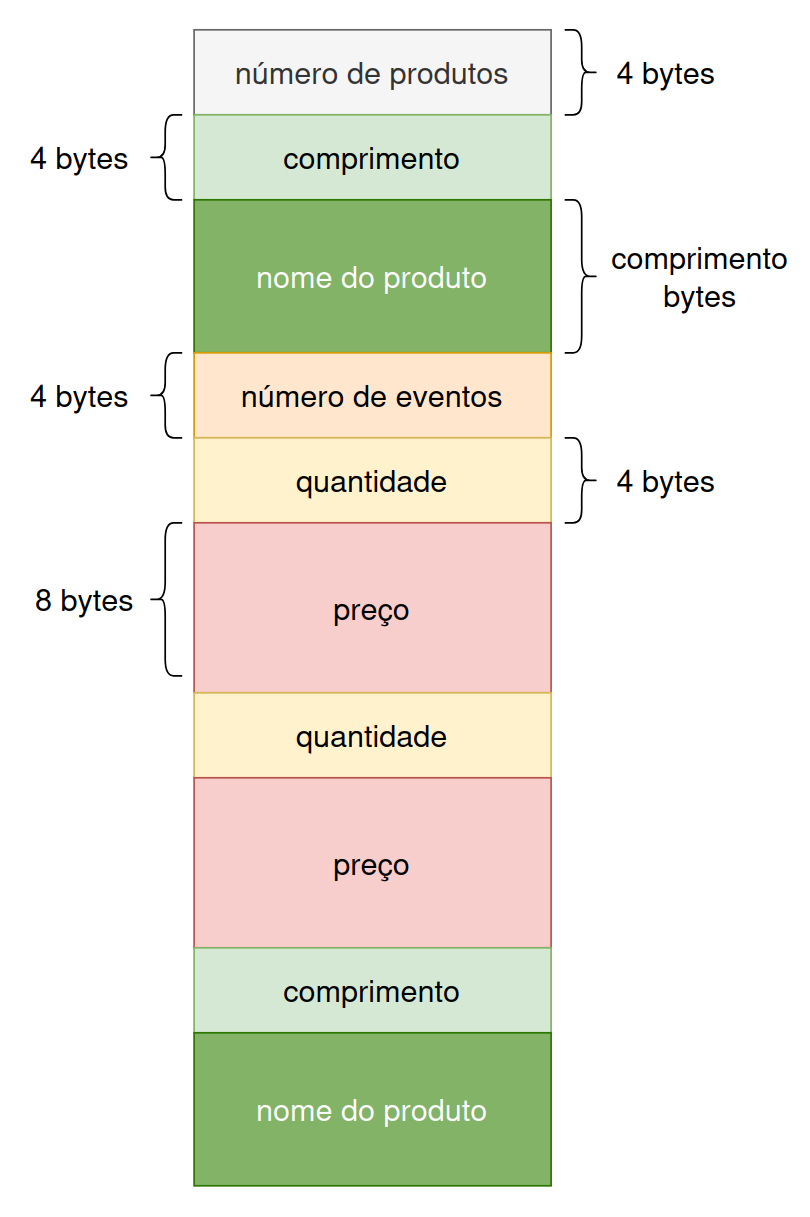
\includegraphics[width=0.7\textwidth]{imgs/serializacao-eficiente.png}}
			\caption{Serialização compacta}
			\label{fig:serializacao-compacta}
			
		\end{minipage}
	\end{figure}
	
	
	\section{Avaliação Experimental}
	
	A validação experimental da solução proposta foi realizada através de uma bateria de testes automatizada, desenvolvida especificamente para submeter o servidor a cenários de carga intensiva e rigorosa. Esta abordagem permitiu simular um ambiente de alta concorrência, instanciando múltiplos clientes simultâneos para avaliar não só a estabilidade e integridade dos dados sob stress, mas também para aferir métricas quantitativas de desempenho fundamentais, como o débito de processamento e a latência de resposta do serviço.
	
	\subsection{Cenários de Teste}
	
	Em conformidade com os requisitos do projeto, foram desenhados cenários específicos para avaliar as duas dimensões críticas do sistema - escalabilidade e robustez - focando-se nas funcionalidades nucleares do serviço:
	\begin{itemize}
		\item \textbf{Registo de Eventos}: avaliou-se o desempenho da operação de adicionar eventos à série temporal do dia corrente (AddEvent). Este cenário testa a capacidade do servidor em gerir a concorrência na escrita de novos dados em tempo real.
		\item \textbf{Agregação de Informação}: avaliou-se o desempenho das operações de consulta sobre dias anteriores (GetStock, GetProfit, GetAverage, GetMax). Estas operações testam a eficácia do processamento lazy (on demand) e do mecanismo de caching implementado, simulando múltiplos clientes a solicitar agregações sobre subconjuntos de produtos e intervalos de dias.
		\item \textbf{Teste de Robustez}: simulou-se um cenário de falha de consumo por parte de um cliente ("cliente lento"), que estabelece conexão mas não lê as respostas enviadas. O objetivo foi verificar se esta situação bloqueia recursos no servidor, impedindo-o de responder a outros clientes ativos.
	\end{itemize}
	
	\subsection{Análide de Resultados}
	
	A tabela \ref{tab:resultados} apresenta os resultados obtidos na execução dos testes nos cenários descritos. A máquina usada para a realização dos testes é a seguinte: ASUS Zenbook, Processador Intel Core i7, 16GiB de Memória, Sistema Operativo Ubuntu 24.04. O servidor recebeu os seguintes \textbf{parâmetros}: 5 dias anteriores, 3 séries em memória, 10 entradas na cache.
	\begin{table}[htbp]
		
		\centering
		\caption{Resultados}
		\label{tab:resultados}
		
		\newcolumntype{Y}{>{\centering\arraybackslash}X}
		
		\begin{tabularx}{\textwidth}{l Y Y Y Y}
			\toprule
			\textbf{Operação} & \textbf{Nr Clientes} & \textbf{Nr Operações} & \textbf{Operações/s} & \textbf{Latência (ms)} \\
			\midrule
			ADD EVENT & 1   & 1000 & 23561.51  & 0.0424 \\
			ADD EVENT & 10  & 1000 & 143693.57 & 0.0594 \\
			ADD EVENT & 50  & 1000 & 483933.47 & 0.0827 \\
			ADD EVENT & 100 & 1000 & 741790.46 & 0.1075 \\
			\midrule
			STOCK & 1   & 100 & 48.24 & 20.7289 \\
			STOCK & 10  & 100 & 78.85 & 121.5372 \\
			STOCK & 50  & 100 & 76.65 & 627.4628 \\
			STOCK & 100 & 100 & 73.85 & 1297.3056 \\
			\midrule
			TOTAL & 1   & 500 & 53.74 & 18.6072 \\
			TOTAL & 10  & 500 & 80.97 & 121.8100 \\
			TOTAL & 50  & 500 & 71.08 & 687.1654 \\
			TOTAL & 100 & 500 & 70.12 & 1334.2131 \\
			\midrule
			AVERAGE & 1   & 1000 & 52.77 & 19.1982 \\
			AVERAGE & 10  & 1000 & 79.07 & 126.5109 \\
			AVERAGE & 50  & 1000 & 71.60 & 637.0004 \\
			AVERAGE & 100 & 1000 & 71.03 & 1204.2000 \\
			\midrule
			MAXIMUM & 1   & 50   & 50.12 & 18.0072 \\
			MAXIMUM & 10  & 100  & 81.88 & 120.5690 \\
			MAXIMUM & 50  & 500  & 69.98 & 651.7004 \\
			MAXIMUM & 100 & 1000 & 72.45 & 1311.6735 \\
			\bottomrule
		\end{tabularx}
		
	\end{table}
	
	A análise dos dados permite retirar as seguintes conclusões, relacionando-as com as opções de desenho da arquitetura:
	\begin{enumerate}
		\item \textbf{Registo de Eventos}: nesta componente verificamos uma diferença perante a agregação de informação, e isso deve-se ao facto de os testes medirem apenas a latência de envio do pedido, e não da computação efetuada pelo servidor. Isto acontece porque o servidor não envia resposta ao cliente, logo do ponto de vista deste a operação é bastante eficiente.
		\item \textbf{Agregação de Informação}: neste conjunto de operações podemos verificar que o número de operações efetuadas por segundo estabeliza ao atingir as centenas de clientes. Estes testes mostram que o servidor está sobre alguma carga e que seria necessário uma maior paralelização, como por exemplo na serialização das séries temporais, dado que operações em disco são mais custosas.
		\item \textbf{Robustez do Serviço}: o teste de robustez foi superado com sucesso ("OK (Passou)"), confirmando que a arquitetura multithreaded isola eficazmente as ligações. O facto de um cliente não consumir as respostas apenas afeta a sua própria conexão (enchendo o buffer TCP), sem degradar o serviço para os restantes utilizadores que continuam a efetuar operações de registo e agregação normalmente.
	\end{enumerate}
	
	É de notar que os testes realizados não são suficientes para validar a eficiência total do servidor, pois não são avaliados o consumo de CPU por parte do servidor. O programa não aparenta mostrar uma grande capacidade de escalabilidade, é esperado que aumentando o número de dias, perca performance. Uma alternativa a solucionar este problema seria paralelizar a serialização das séries temporais, pois deverá ser uma das operações mais "pesadas" no servidor.
	
	\section{Como Executar}
	
	O programa é composto por 4 executáveis: \texttt{SalesTraceClientMain.java} que apresenta a interface ao utilizador, \texttt{SalesTraceServerMain.java} que inicia o servidor e recebe como parâmetros o número de dias passados, o número máximo de séries em memória, o número máximo de agregações em cache e caminho para a diretoria que contém os dias anteriores em disco. \texttt{GenerateDays.java} é um script que gera um número (especificado) de dias anteriores com eventos aleatórios e \texttt{Tests.java} é um script que executa os testes, discutidos anteriormente, e recebe como parâmetro o número de dias passados.
	
	Para executar a interface do utilizador e os testes de performance é necessário iniciar o servidor primeiramente. O script de geração de dias é independente dos restantes scripts.
	
	\section{Conclusão}
	
	Neste trabalho prático foi desenvolvido um serviço distribuído para o registo e consulta de eventos em séries temporais, suportando operações de agregação, filtragem e notificação de ocorrências. A implementação permitiu aplicar conceitos centrais de Sistemas Distribuídos, nomeadamente concorrência, sincronização entre threads e comunicação cliente-servidor.
	
	A arquitetura cliente-servidor, com um servidor multithreaded, permitiu suportar múltiplos clientes concorrentes de forma eficiente. A separação entre dados do dia corrente e dados históricos garantiu consistência e possibilitou operações de leitura paralelas e escaláveis.
	
	Decisões como a avaliação lazy das agregações, a utilização de uma cache LRU e a serialização compacta de dados contribuíram para a redução do custo computacional e da comunicação. As notificações foram implementadas com base em variáveis de condição, permitindo operações bloqueantes sem precisar de uma espera ativa.
	
	Os resultados experimentais obtidos confirmam que o sistema apresenta um comportamento escalável, eficiente e robusto, estando alinhado com os princípios fundamentais de sistemas distribuídos. Apesar dos resultados obtidos, um ponto a melhorar seria a realização de testes mais realistas, de forma a verificar a verdadeita performance do sistema.
	
	
\end{document}
